\UseRawInputEncoding
\documentclass[12pt,a4paper]{report}

% ======================== PACKAGES ========================
\usepackage[utf8]{inputenc}
\usepackage[T1]{fontenc}
\usepackage[english]{babel}
\usepackage{geometry}
\usepackage{graphicx}
\usepackage{xcolor}
\usepackage{titlesec}
\usepackage{fancyhdr}
\usepackage{hyperref}
\usepackage{listings}
\usepackage{booktabs}
\usepackage{longtable}
\usepackage{enumitem}
\usepackage{tikz}
\usetikzlibrary{shapes.geometric,shapes.multipart,positioning,arrows.meta}
\usepackage{float}
\usepackage{caption}
\usepackage{array}
\usepackage{tabularx}
\usepackage{setspace}
\usepackage{tocloft}
\usepackage{pdfpages}
\usepackage{parskip}

% ======================== PAGE SETUP ========================
\geometry{
  top=2.5cm,
  bottom=2.5cm,
  left=3cm,
  right=2.5cm
}

% ======================== COLORS ========================
\definecolor{primaryorange}{HTML}{F97316}
\definecolor{darkbg}{HTML}{09090B}
\definecolor{codebg}{HTML}{1C1C1C}
\definecolor{codetext}{HTML}{E5E7EB}
\definecolor{commentgreen}{HTML}{6A9955}
\definecolor{keywordblue}{HTML}{569CD6}
\definecolor{stringorange}{HTML}{CE9178}

% ======================== HYPERREF ========================
\hypersetup{
  colorlinks=true,
  linkcolor=primaryorange,
  urlcolor=primaryorange,
  citecolor=primaryorange,
  pdfauthor={CyberStore Team},
  pdftitle={CyberStore E-Commerce Platform - Final Project Report},
  pdfsubject={Software Engineering Final Project},
}

% ======================== CODE LISTINGS ========================
\lstset{
  backgroundcolor=\color{codebg},
  basicstyle=\ttfamily\small\color{codetext},
  keywordstyle=\color{keywordblue}\bfseries,
  commentstyle=\color{commentgreen}\itshape,
  stringstyle=\color{stringorange},
  breaklines=true,
  frame=single,
  rulecolor=\color{gray!40},
  numbers=left,
  numberstyle=\tiny\color{gray},
  numbersep=8pt,
  tabsize=2,
  showstringspaces=false,
  captionpos=b,
  xleftmargin=1.5em,
  framexleftmargin=1.5em,
}

\lstdefinelanguage{JavaScript}{
  keywords={const, let, var, function, return, if, else, for, while, class, static, async, await, try, catch, finally, import, export, default, from, new, this, typeof, instanceof},
  morecomment=[l]{//},
  morecomment=[s]{/*}{*/},
  morestring=[b]',
  morestring=[b]",
  morestring=[b]`,
  sensitive=true,
}

% ======================== HEADERS & FOOTERS ========================
\pagestyle{fancy}
\fancyhf{}
\fancyhead[L]{\small\textcolor{gray}{CyberStore -- Final Project Report}}
\fancyhead[R]{\small\textcolor{gray}{\leftmark}}
\fancyfoot[C]{\thepage}
\renewcommand{\headrulewidth}{0.4pt}
\renewcommand{\footrulewidth}{0pt}

% ======================== CHAPTER TITLE FORMAT ========================
\titleformat{\chapter}[display]
  {\normalfont\huge\bfseries\color{primaryorange}}
  {\chaptertitlename\ \thechapter}{20pt}{\Huge}
\titlespacing*{\chapter}{0pt}{-20pt}{30pt}

% ======================== DOCUMENT ========================
\begin{document}

% ======================= TITLE PAGE =======================
\begin{titlepage}
  \begin{center}
    \vspace*{1cm}

    {\Large\textsc{University Name}}\\[0.3cm]
    {\large Faculty of Computer Science \& Information Technology}\\[0.3cm]
    {\large Department of Software Engineering}\\[1.5cm]

    \rule{\linewidth}{0.5pt}\\[0.6cm]
    {\Huge\bfseries\textcolor{primaryorange}{CyberStore}}\\[0.3cm]
    {\LARGE\bfseries Full-Stack E-Commerce Platform}\\[0.2cm]
    \rule{\linewidth}{0.5pt}\\[2cm]

    {\Large\textbf{Final Year Graduation Project Report}}\\[0.5cm]
    {\large Last Cycle -- Academic Year 2025/2026}\\[2cm]

    \begin{minipage}{0.45\textwidth}
      \begin{flushleft}
        \textbf{Prepared by:}\\[0.3cm]
        Student Name\\
        Student ID: XXXXXXXXX
      \end{flushleft}
    \end{minipage}
    \hfill
    \begin{minipage}{0.45\textwidth}
      \begin{flushright}
        \textbf{Supervised by:}\\[0.3cm]
        Dr.~Supervisor Name\\
        Department of Software Engineering
      \end{flushright}
    \end{minipage}

    \vfill
    {\large March 2026}
  \end{center}
\end{titlepage}

% ======================= ABSTRACT =======================
\chapter*{Abstract}
\addcontentsline{toc}{chapter}{Abstract}

CyberStore is a modern, full-stack e-commerce web application designed and developed as a final year graduation project. The platform provides a complete online shopping experience for gaming hardware and computer components, featuring a cyberpunk-themed user interface with full bilingual support (English and Arabic).

The system is built using a three-tier architecture: a React.js frontend with Tailwind CSS for responsive UI, a Node.js/Express.js RESTful API backend, and a MySQL relational database. Key features include user authentication with JWT, product catalog with advanced filtering and search, shopping cart management, order processing, supplier management, product reviews and ratings, an admin dashboard for full CRUD operations, and internationalization (i18n) support.

This report documents the complete software development lifecycle of the project, covering requirements analysis, system design, implementation details, database schema, API architecture, and the technologies employed.

\textbf{Keywords:} E-Commerce, React.js, Node.js, Express.js, MySQL, REST API, JWT Authentication, Tailwind CSS, Zustand, Internationalization, Full-Stack Web Development.

% ======================= TABLE OF CONTENTS =======================
\tableofcontents
\listoffigures
\listoftables

% ======================= CHAPTER 1: INTRODUCTION =======================
\chapter{Introduction}

\section{Project Overview}
CyberStore is a comprehensive e-commerce web application built as a graduation project to demonstrate proficiency in modern full-stack web development. The platform specializes in gaming hardware and computer components, providing a sleek cyberpunk-themed user interface that enhances the shopping experience.

The application follows a client--server architecture, with a decoupled React.js single-page application (SPA) communicating with a Node.js/Express.js RESTful API, backed by a MySQL relational database management system.

\section{Problem Statement}
Traditional e-commerce platforms often suffer from:
\begin{itemize}[noitemsep]
  \item Lack of bilingual support (especially Arabic RTL layout)
  \item Poor admin management interfaces for products, orders, users, and suppliers
  \item Absence of supplier relationship management integrated within the e-commerce workflow
  \item Slow, non-responsive user interfaces that do not leverage modern frontend frameworks
  \item Lack of real-time product reviews and rating systems
\end{itemize}

CyberStore addresses these challenges by providing a modern, performant, and feature-rich e-commerce solution with full bilingual support and comprehensive admin tools.

\section{Project Objectives}
The main objectives of this project are:
\begin{enumerate}[noitemsep]
  \item Design and develop a full-stack e-commerce web application using modern technologies.
  \item Implement a responsive, accessible, and visually appealing user interface.
  \item Build a secure RESTful API with JWT-based authentication and role-based access control.
  \item Design a normalized relational database schema for products, orders, users, suppliers, reviews, and categories.
  \item Implement full CRUD operations for an admin dashboard.
  \item Support bilingual content (English and Arabic) with RTL layout switching.
  \item Integrate a supplier management system linked to products.
  \item Implement product reviews and ratings.
\end{enumerate}

\section{Project Scope}
The project scope includes:
\begin{itemize}[noitemsep]
  \item \textbf{Frontend:} 20+ pages/views including Home, Products, Product Detail, Cart, Checkout, Profile, Login, Register, Categories, Suppliers, Supplier Detail, and Admin pages.
  \item \textbf{Backend:} RESTful API with 7 route groups (auth, products, orders, users, admin, stats, suppliers).
  \item \textbf{Database:} 7 tables (users, categories, suppliers, products, orders, order\_items, reviews).
  \item \textbf{Admin Panel:} Dashboard with statistics, product management, order management, user management, and supplier management.
  \item \textbf{i18n:} Full English and Arabic translations (~1500+ translation keys).
\end{itemize}

\section{Report Structure}
This report is organized as follows:
\begin{itemize}[noitemsep]
  \item \textbf{Chapter 2:} Literature Review and Related Work
  \item \textbf{Chapter 3:} System Analysis and Requirements
  \item \textbf{Chapter 4:} System Design and Architecture
  \item \textbf{Chapter 5:} Implementation and Technologies
  \item \textbf{Chapter 6:} Database Design
  \item \textbf{Chapter 7:} API Design
  \item \textbf{Chapter 8:} User Interface
  \item \textbf{Chapter 9:} Testing and Evaluation
  \item \textbf{Chapter 10:} Conclusion and Future Work
\end{itemize}


% ======================= CHAPTER 2: LITERATURE REVIEW =======================
\chapter{Literature Review and Related Work}

\section{E-Commerce Systems}
Electronic commerce (e-commerce) has revolutionized the retail industry by enabling businesses and consumers to conduct transactions over the internet. Modern e-commerce platforms such as Shopify, WooCommerce, and Amazon use sophisticated architectures with microservices, CDNs, and advanced search capabilities.

Key requirements for a successful e-commerce platform include:
\begin{itemize}[noitemsep]
  \item Secure user authentication and authorization
  \item Product catalog with search and filtering
  \item Shopping cart and checkout workflows
  \item Order management and tracking
  \item Responsive design for mobile and desktop
  \item Performance optimization and scalability
\end{itemize}

\section{Single-Page Applications (SPA)}
Single-Page Applications load a single HTML page and dynamically update content as the user interacts with the application. React.js, developed by Meta (Facebook), is one of the most widely adopted libraries for building SPAs. Its component-based architecture, virtual DOM, and rich ecosystem make it ideal for building complex, interactive user interfaces.

\section{RESTful API Architecture}
REST (Representational State Transfer) is an architectural style for designing networked applications. RESTful APIs use HTTP methods (GET, POST, PUT, DELETE) to perform CRUD operations on resources identified by URIs. Express.js is the de facto standard for building RESTful APIs in the Node.js ecosystem due to its minimalistic, unopinionated design.

\section{Related Work}
\begin{table}[H]
\centering
\caption{Comparison with Related E-Commerce Projects}
\label{tab:related}
\begin{tabularx}{\textwidth}{|l|X|X|X|}
\hline
\textbf{Feature} & \textbf{ProShop (MERN)} & \textbf{Shopify Starter} & \textbf{CyberStore (Ours)} \\
\hline
Frontend & React + Bootstrap & Liquid Templates & React + Tailwind CSS \\
\hline
Backend & Node/Express & Ruby on Rails & Node/Express \\
\hline
Database & MongoDB & PostgreSQL & MySQL \\
\hline
i18n Support & No & Partial & Full (EN/AR + RTL) \\
\hline
Supplier Mgmt & No & No & Yes \\
\hline
Reviews & Basic & Plugin-based & Built-in \\
\hline
Admin Panel & Basic & Full & Full (5 modules) \\
\hline
Animations & No & Minimal & Framer Motion \\
\hline
\end{tabularx}
\end{table}


% ======================= CHAPTER 3: REQUIREMENTS =======================
\chapter{System Analysis and Requirements}

\section{Functional Requirements}

\subsection{User Management}
\begin{itemize}[noitemsep]
  \item FR-01: Users can register with name, email, and password.
  \item FR-02: Users can log in and receive a JWT token.
  \item FR-03: Users can view and update their profile.
  \item FR-04: Admin users can view, edit, and delete user accounts.
\end{itemize}

\subsection{Product Management}
\begin{itemize}[noitemsep]
  \item FR-05: Users can browse products with pagination, sorting, and filtering.
  \item FR-06: Users can search products by name or description (full-text search).
  \item FR-07: Users can view product details including features, specifications, and reviews.
  \item FR-08: Admin can create, edit, and delete products.
  \item FR-09: Products can be assigned to categories and suppliers.
  \item FR-10: Users can submit reviews and ratings for products.
\end{itemize}

\subsection{Shopping Cart and Orders}
\begin{itemize}[noitemsep]
  \item FR-11: Users can add/remove products from the cart.
  \item FR-12: Users can proceed to checkout and place orders.
  \item FR-13: Users can view their order history.
  \item FR-14: Admin can view all orders and update order status.
\end{itemize}

\subsection{Supplier Management}
\begin{itemize}[noitemsep]
  \item FR-15: Public supplier listing and detail pages.
  \item FR-16: Admin can create, edit, delete, and toggle supplier status.
  \item FR-17: Suppliers linked to products via foreign key.
  \item FR-18: Supplier details include contact, address, and financial information.
\end{itemize}

\subsection{Internationalization}
\begin{itemize}[noitemsep]
  \item FR-19: Full English and Arabic language support.
  \item FR-20: Automatic RTL/LTR layout switching.
  \item FR-21: Language toggle accessible from the navigation bar.
\end{itemize}

\section{Non-Functional Requirements}
\begin{itemize}[noitemsep]
  \item NFR-01: \textbf{Performance} -- Page load time under 3 seconds.
  \item NFR-02: \textbf{Security} -- Passwords hashed with bcrypt; JWT-based auth with expiration.
  \item NFR-03: \textbf{Responsiveness} -- Fully responsive design for mobile, tablet, and desktop.
  \item NFR-04: \textbf{Usability} -- Intuitive navigation and consistent design patterns.
  \item NFR-05: \textbf{Scalability} -- Database connection pooling; modular code structure.
  \item NFR-06: \textbf{Maintainability} -- Separation of concerns; component-based architecture.
\end{itemize}

\section{Use Cases}

\subsection{Use Case Diagram Description}
The system supports three primary actors:
\begin{enumerate}[noitemsep]
  \item \textbf{Guest} -- Can browse products, view suppliers, register, and login.
  \item \textbf{Authenticated User} -- Can manage cart, place orders, write reviews, and manage profile.
  \item \textbf{Admin} -- Can manage all resources (products, orders, users, suppliers) via the dashboard.
\end{enumerate}

\begin{table}[H]
\centering
\caption{Key Use Cases}
\label{tab:usecases}
\begin{tabularx}{\textwidth}{|l|l|X|}
\hline
\textbf{ID} & \textbf{Actor} & \textbf{Use Case} \\
\hline
UC-01 & Guest & Register a new account \\
UC-02 & Guest & Browse and search products \\
UC-03 & User & Add product to shopping cart \\
UC-04 & User & Place an order (checkout) \\
UC-05 & User & Submit a product review \\
UC-06 & User & View order history \\
UC-07 & Admin & Add/Edit/Delete products \\
UC-08 & Admin & Manage orders (view, confirm, reject) \\
UC-09 & Admin & Manage users (view, edit, delete) \\
UC-10 & Admin & Manage suppliers (CRUD, toggle active) \\
UC-11 & Any & Switch language (EN/AR) \\
\hline
\end{tabularx}
\end{table}

\subsection{Use Case Diagram}
Figure~\ref{fig:usecase} illustrates the use case diagram showing the three actors and their interactions with the system.

\begin{figure}[H]
\centering
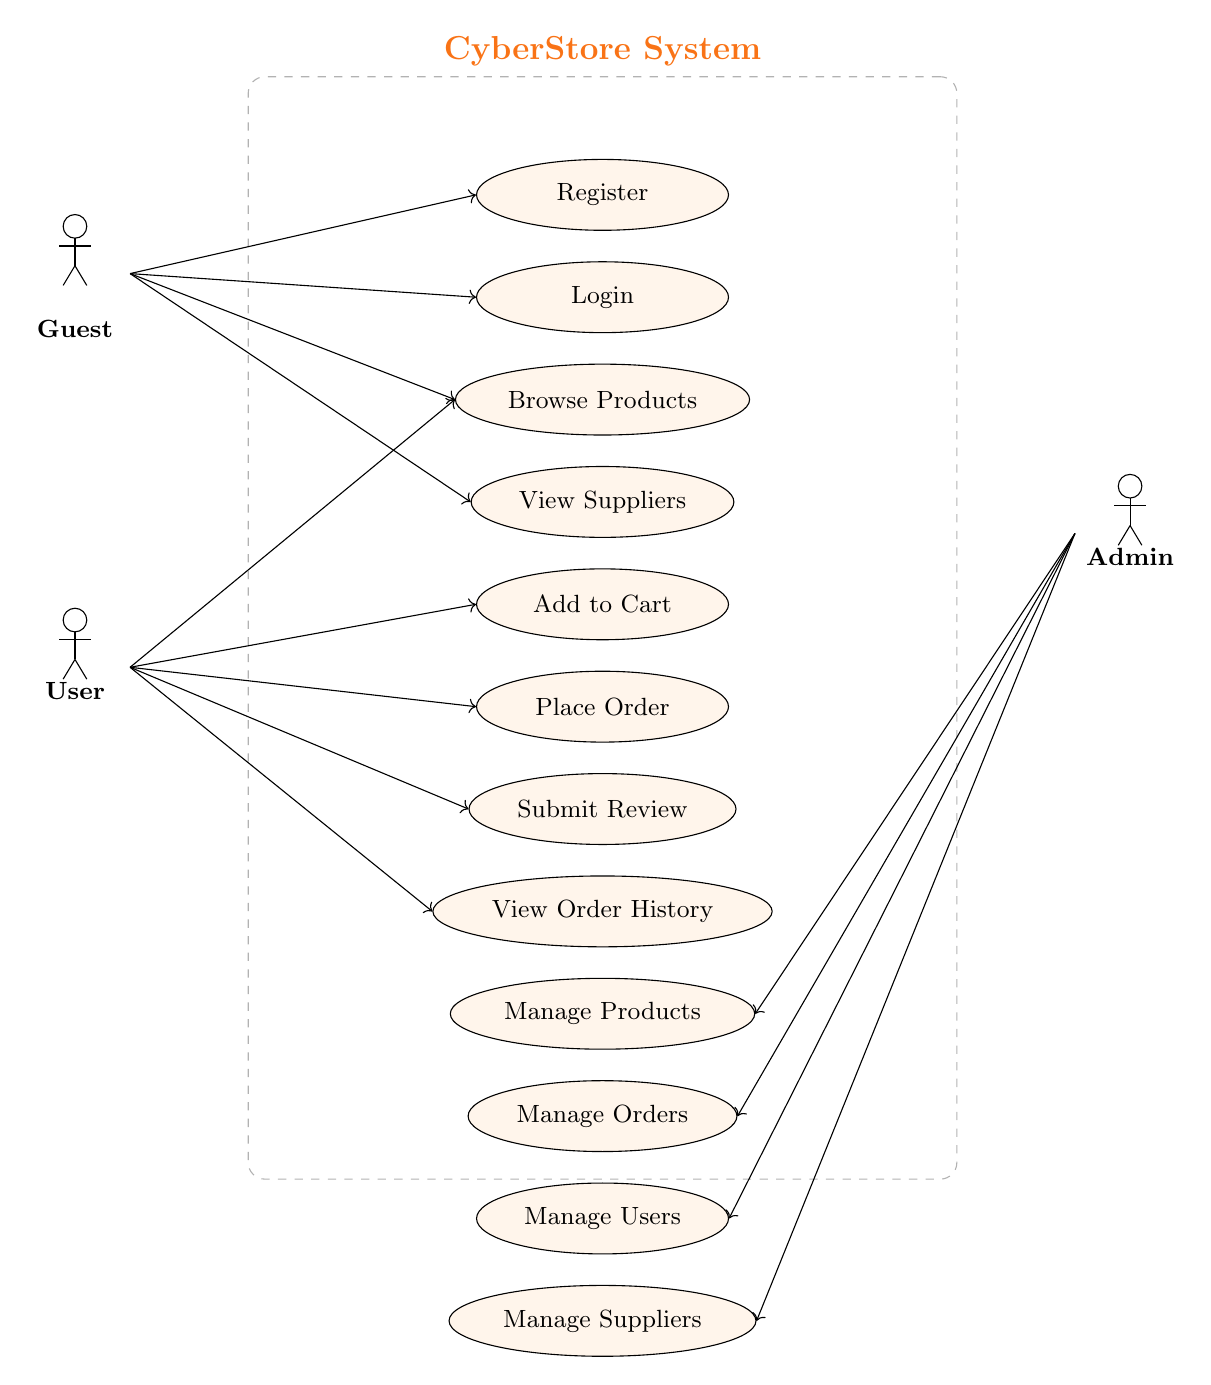
\begin{tikzpicture}[
  actor/.style={font=\small\bfseries, align=center},
  usecase/.style={draw, ellipse, minimum width=3.2cm, minimum height=0.9cm, font=\small, align=center, fill=orange!8},
  sysbox/.style={draw, rounded corners=6pt, minimum width=9cm, minimum height=14cm, dashed, gray!60},
]
  % System boundary
  \node[sysbox, label={[font=\bfseries\large, primaryorange]above:CyberStore System}] (sys) at (4.5,0) {};

  % Actors (stick figures via labels)
  \node[actor] at (-2.2, 4.8) {\tikz{\draw (0,0.4) circle(0.15); \draw (0,0.25) -- (0,-0.1); \draw (-0.2,0.15) -- (0.2,0.15); \draw (0,-0.1) -- (-0.15,-0.35); \draw (0,-0.1) -- (0.15,-0.35);}};
  \node[actor] at (-2.2, 3.8) {Guest};

  \node[actor] at (-2.2, -0.2) {\tikz{\draw (0,0.4) circle(0.15); \draw (0,0.25) -- (0,-0.1); \draw (-0.2,0.15) -- (0.2,0.15); \draw (0,-0.1) -- (-0.15,-0.35); \draw (0,-0.1) -- (0.15,-0.35);}};
  \node[actor] at (-2.2, -0.8) {User};

  \node[actor] at (11.2, 1.5) {\tikz{\draw (0,0.4) circle(0.15); \draw (0,0.25) -- (0,-0.1); \draw (-0.2,0.15) -- (0.2,0.15); \draw (0,-0.1) -- (-0.15,-0.35); \draw (0,-0.1) -- (0.15,-0.35);}};
  \node[actor] at (11.2, 0.9) {Admin};

  % Use cases
  \node[usecase] (uc1) at (4.5, 5.5) {Register};
  \node[usecase] (uc2) at (4.5, 4.2) {Login};
  \node[usecase] (uc3) at (4.5, 2.9) {Browse Products};
  \node[usecase] (uc4) at (4.5, 1.6) {View Suppliers};
  \node[usecase] (uc5) at (4.5, 0.3) {Add to Cart};
  \node[usecase] (uc6) at (4.5, -1.0) {Place Order};
  \node[usecase] (uc7) at (4.5, -2.3) {Submit Review};
  \node[usecase] (uc8) at (4.5, -3.6) {View Order History};
  \node[usecase] (uc9) at (4.5, -4.9) {Manage Products};
  \node[usecase] (uc10) at (4.5, -6.2) {Manage Orders};
  \node[usecase] (uc11) at (4.5, -7.5) {Manage Users};
  \node[usecase] (uc12) at (4.5, -8.8) {Manage Suppliers};

  % Guest connections
  \draw[->] (-1.5, 4.5) -- (uc1.west);
  \draw[->] (-1.5, 4.5) -- (uc2.west);
  \draw[->] (-1.5, 4.5) -- (uc3.west);
  \draw[->] (-1.5, 4.5) -- (uc4.west);

  % User connections
  \draw[->] (-1.5, -0.5) -- (uc3.west);
  \draw[->] (-1.5, -0.5) -- (uc5.west);
  \draw[->] (-1.5, -0.5) -- (uc6.west);
  \draw[->] (-1.5, -0.5) -- (uc7.west);
  \draw[->] (-1.5, -0.5) -- (uc8.west);

  % Admin connections
  \draw[->] (10.5, 1.2) -- (uc9.east);
  \draw[->] (10.5, 1.2) -- (uc10.east);
  \draw[->] (10.5, 1.2) -- (uc11.east);
  \draw[->] (10.5, 1.2) -- (uc12.east);

\end{tikzpicture}
\caption{Use Case Diagram}
\label{fig:usecase}
\end{figure}


% ======================= CHAPTER 4: SYSTEM DESIGN =======================
\chapter{System Design and Architecture}

\section{System Architecture}
CyberStore follows a \textbf{three-tier architecture}:

\begin{enumerate}[noitemsep]
  \item \textbf{Presentation Tier (Frontend):} React.js SPA served on port 5173/3000, communicating with the backend via HTTP/REST.
  \item \textbf{Application Tier (Backend):} Node.js/Express.js server on port 5000, exposing RESTful API endpoints.
  \item \textbf{Data Tier (Database):} MySQL 8.x relational database on port 3306.
\end{enumerate}

\begin{figure}[H]
\centering
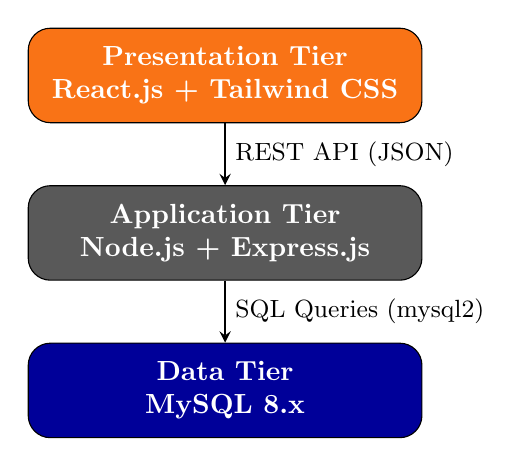
\begin{tikzpicture}[
  box/.style={draw, rounded corners=8pt, minimum width=5cm, minimum height=1.2cm, font=\bfseries, text=white, align=center},
  arrow/.style={->, thick, >=stealth}
]
  \node[box, fill=primaryorange] (fe) at (0,4) {Presentation Tier\\React.js + Tailwind CSS};
  \node[box, fill=gray!70!black] (be) at (0,2) {Application Tier\\Node.js + Express.js};
  \node[box, fill=blue!60!black] (db) at (0,0) {Data Tier\\MySQL 8.x};

  \draw[arrow] (fe) -- node[right, font=\small] {REST API (JSON)} (be);
  \draw[arrow] (be) -- node[right, font=\small] {SQL Queries (mysql2)} (db);
\end{tikzpicture}
\caption{Three-Tier System Architecture}
\label{fig:architecture}
\end{figure}

\section{Frontend Architecture}
The frontend follows a component-based architecture:

\begin{itemize}[noitemsep]
  \item \textbf{Pages (20+):} Home, Products, ProductDetail, Cart, Checkout, Login, Register, Profile, Categories, Suppliers, SupplierDetail, About, Contact, Support, NewArrivals, Trending, Sale, PreOrder, TrackOrder, OrderConfirmation.
  \item \textbf{Admin Pages (8):} Dashboard (with Overview, Products, Orders, Users, Suppliers tabs), AddProduct, AddSupplier, AdminLogin, ProductsManager, OrdersManager, UsersManager, SuppliersManager.
  \item \textbf{Components:} CyberNavbar, ProductCard, Footer, TerminalAnimation.
  \item \textbf{State Management:} Zustand stores -- \texttt{authStore} (authentication), \texttt{cartStore} (shopping cart), \texttt{langStore} (language/i18n).
  \item \textbf{Services:} Centralized Axios API client (\texttt{api.js}) with interceptors for auth tokens and error handling.
\end{itemize}

\section{Backend Architecture}
The backend follows the MVC (Model--View--Controller) pattern:

\begin{itemize}[noitemsep]
  \item \textbf{Routes (7 modules):} auth, products, orders, users, admin, stats, suppliers.
  \item \textbf{Controllers (6):} authController, productController, orderController, userController, adminController, supplierController, statsController.
  \item \textbf{Models (7):} User, Product, Category, Order, OrderItem, Review, Supplier.
  \item \textbf{Middleware:} JWT authentication (\texttt{protect}), admin authorization (\texttt{admin}), error handling.
  \item \textbf{Config:} Database connection pool with auto-migration (table creation and schema updates).
\end{itemize}

\section{Class Diagram}
Figure~\ref{fig:classdiagram} shows the main backend model classes with their attributes, methods, and relationships.

% --- UML class box helper macro ---
% \umlclass{nodename}{x}{y}{ClassName}{attributes}{methods}
\newcommand{\umlclass}[6]{%
  \node[
    draw=gray!60, thick, rectangle split, rectangle split parts=3,
    rectangle split part fill={orange!25, white, blue!6},
    rounded corners=4pt,
    font=\small,
    minimum width=4.8cm,
    text width=4.6cm,
  ] (#1) at (#2,#3) {
    \textbf{#4}
    \nodepart{second}
    \begin{tabular}{@{}l@{}}
      #5
    \end{tabular}
    \nodepart{third}
    \begin{tabular}{@{}l@{}}
      #6
    \end{tabular}
  };%
}

\begin{figure}[H]
\centering
\resizebox{\textwidth}{!}{
\begin{tikzpicture}[
  rel/.style={->, thick, >=stealth, draw=gray!70},
  drel/.style={->, thick, >=stealth, dashed, draw=gray!60},
  lbl/.style={font=\scriptsize\bfseries, fill=white, inner sep=1pt},
]

% ---- Row 1: User  |  Product  |  Category ----
\umlclass{User}{0}{0}{User}{%
  \texttt{+ id: INT \ \ [PK]}\\
  \texttt{+ username: VARCHAR(50)}\\
  \texttt{+ email: VARCHAR(100)}\\
  \texttt{- password: VARCHAR}\\
  \texttt{+ role: ENUM(user,admin)}\\
  \texttt{+ balance: DECIMAL}\\
  \texttt{+ is\_active: BOOLEAN}\\
  \texttt{+ created\_at: TIMESTAMP}
}{%
  \texttt{+ findByEmail(email)}\\
  \texttt{+ create(data)}\\
  \texttt{+ findAll(page)}\\
  \texttt{+ update(id, data)}\\
  \texttt{+ delete(id)}
}

\umlclass{Product}{7}{0}{Product}{%
  \texttt{+ id: INT \ \ [PK]}\\
  \texttt{+ name: VARCHAR(200)}\\
  \texttt{+ slug: VARCHAR \ [UNIQUE]}\\
  \texttt{+ price: DECIMAL(10,2)}\\
  \texttt{+ stock: INT}\\
  \texttt{+ sku: VARCHAR(50) [UNIQUE]}\\
  \texttt{+ rating: DECIMAL(3,2)}\\
  \texttt{+ category\_id: INT \ [FK]}\\
  \texttt{+ supplier\_id: INT \ [FK]}\\
  \texttt{+ is\_featured: BOOLEAN}\\
  \texttt{+ is\_active: BOOLEAN}
}{%
  \texttt{+ findAll(filters)}\\
  \texttt{+ findById(id)}\\
  \texttt{+ findBySlug(slug)}\\
  \texttt{+ create(data)}\\
  \texttt{+ update(id, data)}\\
  \texttt{+ delete(id)}
}

\umlclass{Category}{14}{0}{Category}{%
  \texttt{+ id: INT \ \ [PK]}\\
  \texttt{+ name: VARCHAR(100)}\\
  \texttt{+ slug: VARCHAR \ [UNIQUE]}\\
  \texttt{+ description: TEXT}\\
  \texttt{+ icon: VARCHAR(50)}\\
  \texttt{+ is\_active: BOOLEAN}
}{%
  \texttt{+ findAll()}\\
  \texttt{+ findById(id)}\\
  \texttt{+ findBySlug(slug)}\\
  \texttt{+ create(data)}\\
  \texttt{+ update(id, data)}
}

% ---- Row 2: Order  |  Review  |  Supplier ----
\umlclass{Order}{0}{-9}{Order}{%
  \texttt{+ id: INT \ \ [PK]}\\
  \texttt{+ user\_id: INT \ [FK]}\\
  \texttt{+ total\_amount: DECIMAL}\\
  \texttt{+ status: VARCHAR(20)}\\
  \texttt{+ shipping\_address: TEXT}\\
  \texttt{+ payment\_method: VARCHAR}\\
  \texttt{+ created\_at: TIMESTAMP}
}{%
  \texttt{+ create(data)}\\
  \texttt{+ findByUser(userId)}\\
  \texttt{+ findAll(filters)}\\
  \texttt{+ updateStatus(id, status)}
}

\umlclass{Review}{7}{-9}{Review}{%
  \texttt{+ id: INT \ \ [PK]}\\
  \texttt{+ product\_id: INT \ [FK]}\\
  \texttt{+ user\_id: INT \ [FK]}\\
  \texttt{+ rating: INT \ (1--5)}\\
  \texttt{+ comment: TEXT}\\
  \texttt{+ created\_at: TIMESTAMP}
}{%
  \texttt{+ create(data)}\\
  \texttt{+ findByProduct(id)}\\
  \texttt{+ findByUser(id)}\\
  \texttt{+ delete(id)}
}

\umlclass{Supplier}{14}{-9}{Supplier}{%
  \texttt{+ id: INT \ \ [PK]}\\
  \texttt{+ name: VARCHAR(200)}\\
  \texttt{+ slug: VARCHAR \ [UNIQUE]}\\
  \texttt{+ email: VARCHAR(100)}\\
  \texttt{+ phone: VARCHAR(50)}\\
  \texttt{+ city: VARCHAR(100)}\\
  \texttt{+ country: VARCHAR(100)}\\
  \texttt{+ rating: DECIMAL(3,2)}\\
  \texttt{+ is\_active: BOOLEAN}
}{%
  \texttt{+ findAll(filters)}\\
  \texttt{+ findById(id)}\\
  \texttt{+ create(data)}\\
  \texttt{+ update(id, data)}\\
  \texttt{+ delete(id)}
}

% ---- Row 3 (centre): OrderItem ----
\umlclass{OrderItem}{3.5}{-18}{OrderItem}{%
  \texttt{+ id: INT \ \ [PK]}\\
  \texttt{+ order\_id: INT \ [FK]}\\
  \texttt{+ product\_id: INT \ [FK]}\\
  \texttt{+ quantity: INT}\\
  \texttt{+ price: DECIMAL(10,2)}
}{%
  \texttt{+ create(data)}\\
  \texttt{+ findByOrder(orderId)}
}

% ========== RELATIONSHIPS ==========

% Product ---N:1---> Category
\draw[rel] (Product.east) -- node[lbl, above] {N:1} node[lbl, below] {category} (Category.west);

% Product ---N:1---> Supplier
\draw[rel] (Product.south east) -- ++(0,-1.2) -- ++(2.5,0) |- node[lbl, near end, right] {N:1} (Supplier.west);

% User ---1:N---> Order
\draw[rel] (User.south) -- ++(0,-0.8) -- ++(-2.3,0) |- node[lbl, near end, left] {1:N} (Order.north west);

% User ---1:N---> Review
\draw[drel] (User.south east) -- ++(0,-0.8) ++ (0,0) -- ++(1,0) |- node[lbl, near end, right] {writes 1:N} (Review.north east);

% Order ---1:N---> OrderItem
\draw[rel] (Order.south) -- ++(0,-0.5) -- ++(-2,0) |- node[lbl, near end, left] {1:N} (OrderItem.north west);

% Product ---1:N---> Review
\draw[rel] (Product.south) -- ++(0,-0.5) -- ++(0.3,0) |- node[lbl, near end, right] {1:N} (Review.north);

% Product ---1:N---> OrderItem
\draw[drel] (Product.south west) -- ++(0,-1.5) -- ++(-2.2,0) |- node[lbl, near end, left] {1:N} (OrderItem.north);

\end{tikzpicture}
}
\caption{Class Diagram -- Backend Models and Relationships}
\label{fig:classdiagram}
\end{figure}

\section{Directory Structure}
\begin{lstlisting}[language={}, caption={Project Directory Structure}]
cyberstore/
  +-- backend/
  |   +-- server.js            # Express app entry point
  |   +-- config/db.js         # MySQL pool + auto-migration
  |   +-- controllers/         # Business logic (6 controllers)
  |   +-- middleware/           # auth.js (JWT + admin)
  |   +-- models/              # Data models (7 models)
  |   +-- routes/              # API routes (7 modules)
  |   +-- scripts/             # Utility & test scripts
  |   +-- public/uploads/      # Uploaded product images
  +-- frontend/
  |   +-- src/
  |   |   +-- App.jsx          # Router + route definitions
  |   |   +-- components/      # Reusable UI components
  |   |   +-- pages/           # Page components (20+)
  |   |   +-- pages/Admin/     # Admin panel (8 components)
  |   |   +-- pages/store/     # Zustand stores (3 stores)
  |   |   +-- services/api.js  # Axios API client
  |   |   +-- i18n/            # translations.js (EN + AR)
  |   +-- public/              # Static assets
  +-- package.json             # Root scripts (concurrently)
\end{lstlisting}


% ======================= CHAPTER 5: IMPLEMENTATION =======================
\chapter{Implementation and Technologies}

\section{Technology Stack}
\begin{table}[H]
\centering
\caption{Technology Stack Summary}
\label{tab:techstack}
\begin{tabularx}{\textwidth}{|l|l|X|}
\hline
\textbf{Layer} & \textbf{Technology} & \textbf{Purpose} \\
\hline
Frontend & React.js 18.2 & Component-based UI library \\
Routing & React Router DOM 6 & Client-side routing and navigation \\
Styling & Tailwind CSS 3.4 & Utility-first CSS framework \\
Animations & Framer Motion 12 & Declarative animations and transitions \\
Icons & Lucide React & Consistent SVG icon library \\
State & Zustand 4.4 & Lightweight state management \\
HTTP Client & Axios 1.6 & HTTP requests with interceptors \\
Charts & Recharts 3.7 & Dashboard statistics visualization \\
\hline
Backend & Node.js & JavaScript runtime environment \\
Framework & Express.js 4.18 & Minimalist web framework \\
Database Driver & mysql2 3.6 & MySQL client with promise support \\
Auth & jsonwebtoken 9.0 & JWT token generation and verification \\
Encryption & bcryptjs 2.4 & Password hashing \\
Environment & dotenv 16.3 & Environment variable management \\
Email & Nodemailer 6.10 & Email sending capability \\
PDF & PDFKit 0.13 & PDF document generation \\
\hline
Database & MySQL 8.x & Relational database management system \\
\hline
Dev Tools & Nodemon 3.0 & Auto-restart on code changes \\
 & Concurrently 8.2 & Run frontend + backend simultaneously \\
 & ESLint & Code linting and quality \\
\hline
\end{tabularx}
\end{table}

\section{Authentication and Security}
\subsection{JWT Authentication Flow}
\begin{enumerate}[noitemsep]
  \item User submits credentials (email + password) via \texttt{POST /api/auth/login}.
  \item Server validates credentials and compares bcrypt-hashed password.
  \item On success, server generates a JWT token containing the user ID.
  \item Token is returned to the client and stored in \texttt{localStorage}.
  \item Subsequent API requests include the token in the \texttt{Authorization: Bearer <token>} header.
  \item The \texttt{protect} middleware verifies the token and attaches the user object to the request.
  \item The \texttt{admin} middleware checks if the user role is \texttt{'admin'}.
\end{enumerate}

\subsection{Security Measures}
\begin{itemize}[noitemsep]
  \item Passwords hashed using \texttt{bcryptjs} with salt rounds.
  \item JWT tokens with configurable expiration.
  \item CORS configuration with whitelisted origins.
  \item Input validation on all API endpoints.
  \item SQL injection prevention via parameterized queries (\texttt{mysql2} prepared statements).
  \item Role-based access control (user vs. admin).
  \item Axios interceptor auto-redirects on 401 responses.
\end{itemize}

\section{State Management with Zustand}
Three Zustand stores power the application state:

\begin{lstlisting}[language=JavaScript, caption={Zustand Store Architecture}]
// authStore.js - Authentication state
const useAuthStore = create((set) => ({
  user: null,
  token: null,
  isAuthenticated: false,
  login: async (email, password) => { /* ... */ },
  register: async (name, email, password) => { /* ... */ },
  logout: () => { /* ... */ },
  isAdmin: () => { /* checks user.role === 'admin' */ },
}));

// cartStore.js - Shopping cart state
const useCartStore = create(persist((set, get) => ({
  items: [],
  addToCart: (product) => { /* ... */ },
  removeFromCart: (id) => { /* ... */ },
  clearCart: () => { /* ... */ },
  getTotal: () => { /* ... */ },
})));

// langStore.js - Internationalization state
const useLangStore = create(persist((set, get) => ({
  lang: 'en',
  toggleLang: () => { /* switches en <-> ar, updates dir */ },
  t: (key) => { /* returns translated string */ },
})));
\end{lstlisting}

\section{Internationalization (i18n)}
The application supports full English and Arabic translations:
\begin{itemize}[noitemsep]
  \item Over 1,500 translation keys organized by page/section.
  \item The \texttt{langStore} provides a \texttt{t(key)} function that retrieves the correct translation.
  \item RTL/LTR layout automatically switches when the language changes.
  \item \texttt{document.documentElement.dir} and \texttt{document.documentElement.lang} are updated.
  \item All user-facing text across 20+ pages is translated.
\end{itemize}

\section{Frontend Routing}
React Router DOM v6 manages all client-side routes:

\begin{table}[H]
\centering
\caption{Application Routes}
\label{tab:routes}
\begin{tabularx}{\textwidth}{|l|l|X|}
\hline
\textbf{Path} & \textbf{Access} & \textbf{Component} \\
\hline
\texttt{/} & Public & Home \\
\texttt{/products} & Public & Products (catalog) \\
\texttt{/products/:id} & Public & ProductDetail \\
\texttt{/categories} & Public & Categories \\
\texttt{/suppliers} & Public & Suppliers \\
\texttt{/suppliers/:id} & Public & SupplierDetail \\
\texttt{/cart} & Public & Cart \\
\texttt{/login} & Public & Login \\
\texttt{/register} & Public & Register \\
\texttt{/about} & Public & About \\
\texttt{/contact} & Public & Contact \\
\texttt{/support} & Public & Support \\
\texttt{/checkout} & Auth & Checkout \\
\texttt{/profile} & Auth & Profile \\
\texttt{/order-confirmation/:id} & Auth & OrderConfirmation \\
\texttt{/admin/login} & Public & AdminLogin \\
\texttt{/admin/dashboard} & Admin & Dashboard \\
\texttt{/admin/products/new} & Admin & AddProduct \\
\texttt{/admin/products/edit/:id} & Admin & AddProduct (edit mode) \\
\texttt{/admin/suppliers/new} & Admin & AddSupplier \\
\texttt{/admin/suppliers/edit/:id} & Admin & AddSupplier (edit mode) \\
\hline
\end{tabularx}
\end{table}


% ======================= CHAPTER 6: DATABASE DESIGN =======================
\chapter{Database Design}

\section{Database Overview}
The application uses MySQL 8.x with the InnoDB engine and \texttt{utf8mb4} character set for full Unicode support (including Arabic text and emojis). The schema consists of 7 tables with foreign key constraints and indexed columns for performance.

\section{Entity-Relationship Description}
\begin{itemize}[noitemsep]
  \item A \textbf{User} can place many \textbf{Orders} (1:N).
  \item An \textbf{Order} contains many \textbf{OrderItems} (1:N).
  \item A \textbf{Product} belongs to one \textbf{Category} (N:1).
  \item A \textbf{Product} can belong to one \textbf{Supplier} (N:1, nullable).
  \item A \textbf{Product} can have many \textbf{Reviews} (1:N).
  \item A \textbf{Review} is written by one \textbf{User} (N:1).
\end{itemize}

\section{Table Schemas}

\begin{longtable}{|l|l|l|p{5cm}|}
\caption{Database Table Schemas} \label{tab:schema} \\
\hline
\textbf{Table} & \textbf{Column} & \textbf{Type} & \textbf{Description} \\
\hline
\endfirsthead
\hline
\textbf{Table} & \textbf{Column} & \textbf{Type} & \textbf{Description} \\
\hline
\endhead
\hline
\endfoot

\texttt{users} & id & INT PK AUTO\_INC & Primary key \\
 & username & VARCHAR(50) UNIQUE & Display name \\
 & email & VARCHAR(100) UNIQUE & Login email \\
 & password & VARCHAR(255) & Bcrypt hash \\
 & role & ENUM('user','admin') & Access level \\
 & balance & DECIMAL(10,2) & Account balance \\
 & is\_active & BOOLEAN & Account status \\
 & created\_at & TIMESTAMP & Registration date \\
\hline

\texttt{categories} & id & INT PK AUTO\_INC & Primary key \\
 & name & VARCHAR(100) UNIQUE & Category name \\
 & slug & VARCHAR(100) UNIQUE & URL-friendly slug \\
 & description & TEXT & Category description \\
 & icon & VARCHAR(50) & Icon identifier \\
 & is\_active & BOOLEAN & Visibility status \\
\hline

\texttt{suppliers} & id & INT PK AUTO\_INC & Primary key \\
 & name & VARCHAR(200) & Business name \\
 & slug & VARCHAR(200) UNIQUE & URL-friendly slug \\
 & description & TEXT & About the supplier \\
 & email & VARCHAR(100) & Contact email \\
 & phone & VARCHAR(50) & Phone number \\
 & mobile & VARCHAR(50) & Mobile number \\
 & website & VARCHAR(255) & Website URL \\
 & contact\_person & VARCHAR(200) & Contact person name \\
 & contact\_first\_name & VARCHAR(100) & First name \\
 & contact\_last\_name & VARCHAR(100) & Last name \\
 & address & VARCHAR(500) & Full address \\
 & street & VARCHAR(200) & Street address \\
 & city & VARCHAR(100) & City \\
 & country & VARCHAR(100) & Country \\
 & commercial\_register & VARCHAR(100) & Commercial register \# \\
 & tax\_number & VARCHAR(100) & Tax/VAT number \\
 & currency & VARCHAR(10) & Default currency \\
 & opening\_balance & DECIMAL(12,2) & Opening balance \\
 & rating & DECIMAL(3,2) & Average rating \\
 & is\_active & BOOLEAN & Active status \\
\hline

\texttt{products} & id & INT PK AUTO\_INC & Primary key \\
 & name & VARCHAR(200) & Product name \\
 & slug & VARCHAR(200) UNIQUE & URL slug \\
 & description & TEXT & Product description \\
 & price & DECIMAL(10,2) & Price in USD \\
 & category\_id & INT FK & Ref: categories(id) \\
 & supplier\_id & INT FK NULL & Ref: suppliers(id) \\
 & stock & INT & Quantity in stock \\
 & sku & VARCHAR(50) UNIQUE & Stock Keeping Unit \\
 & features & JSON & Feature list \\
 & specifications & JSON & Key-value specs \\
 & image & VARCHAR(255) & Image path \\
 & rating & DECIMAL(3,2) & Average rating \\
 & is\_featured & BOOLEAN & Featured flag \\
 & is\_active & BOOLEAN & Active/deleted \\
\hline

\texttt{orders} & id & INT PK AUTO\_INC & Primary key \\
 & user\_id & INT FK & Ref: users(id) \\
 & total\_amount & DECIMAL(10,2) & Order total \\
 & status & VARCHAR(20) & pending/completed/etc \\
 & shipping\_address & TEXT & Delivery address \\
 & payment\_method & VARCHAR(50) & Payment type \\
\hline

\texttt{order\_items} & id & INT PK AUTO\_INC & Primary key \\
 & order\_id & INT FK & Ref: orders(id) CASCADE \\
 & product\_id & INT FK & Ref: products(id) \\
 & quantity & INT & Item quantity \\
 & price & DECIMAL(10,2) & Price at purchase time \\
\hline

\texttt{reviews} & id & INT PK AUTO\_INC & Primary key \\
 & product\_id & INT FK & Ref: products(id) \\
 & user\_id & INT FK & Ref: users(id) \\
 & rating & INT & 1--5 star rating \\
 & comment & TEXT & Review text \\
 & created\_at & TIMESTAMP & Review date \\
\hline

\end{longtable}

\section{Indexes and Performance}
The database employs the following indexing strategy:
\begin{itemize}[noitemsep]
  \item \textbf{Primary indexes} on all \texttt{id} columns (clustered).
  \item \textbf{Unique indexes} on \texttt{email}, \texttt{username}, \texttt{slug}, \texttt{sku}.
  \item \textbf{Foreign key indexes} on \texttt{category\_id}, \texttt{supplier\_id}, \texttt{user\_id}, \texttt{order\_id}, \texttt{product\_id}.
  \item \textbf{Composite indexes} on \texttt{is\_active}, \texttt{is\_featured}, \texttt{status}, \texttt{price}.
  \item \textbf{Full-text index} on \texttt{products(name, description, sku)} for search.
  \item \textbf{Connection pooling} with 10 concurrent connections via \texttt{mysql2}.
\end{itemize}

\section{Auto-Migration}
The application implements an auto-migration system in \texttt{config/db.js}:
\begin{itemize}[noitemsep]
  \item On startup, \texttt{CREATE TABLE IF NOT EXISTS} ensures all tables exist.
  \item \texttt{ALTER TABLE} commands add new columns to existing tables (e.g., \texttt{supplier\_id} on products).
  \item Errors for already-existing columns are silently ignored, making migrations idempotent.
\end{itemize}


% ======================= CHAPTER 7: API DESIGN =======================
\chapter{API Design}

\section{API Overview}
The backend exposes a RESTful API at \texttt{http://localhost:5000/api/}. All endpoints return JSON responses. Authentication is handled via JWT Bearer tokens in the \texttt{Authorization} header.

\section{Sequence Diagrams}
The following sequence diagrams illustrate key interaction flows.

\subsection{User Authentication Flow}
Figure~\ref{fig:seq-auth} shows the login and JWT authentication sequence.

\begin{figure}[H]
\centering
\resizebox{\textwidth}{!}{
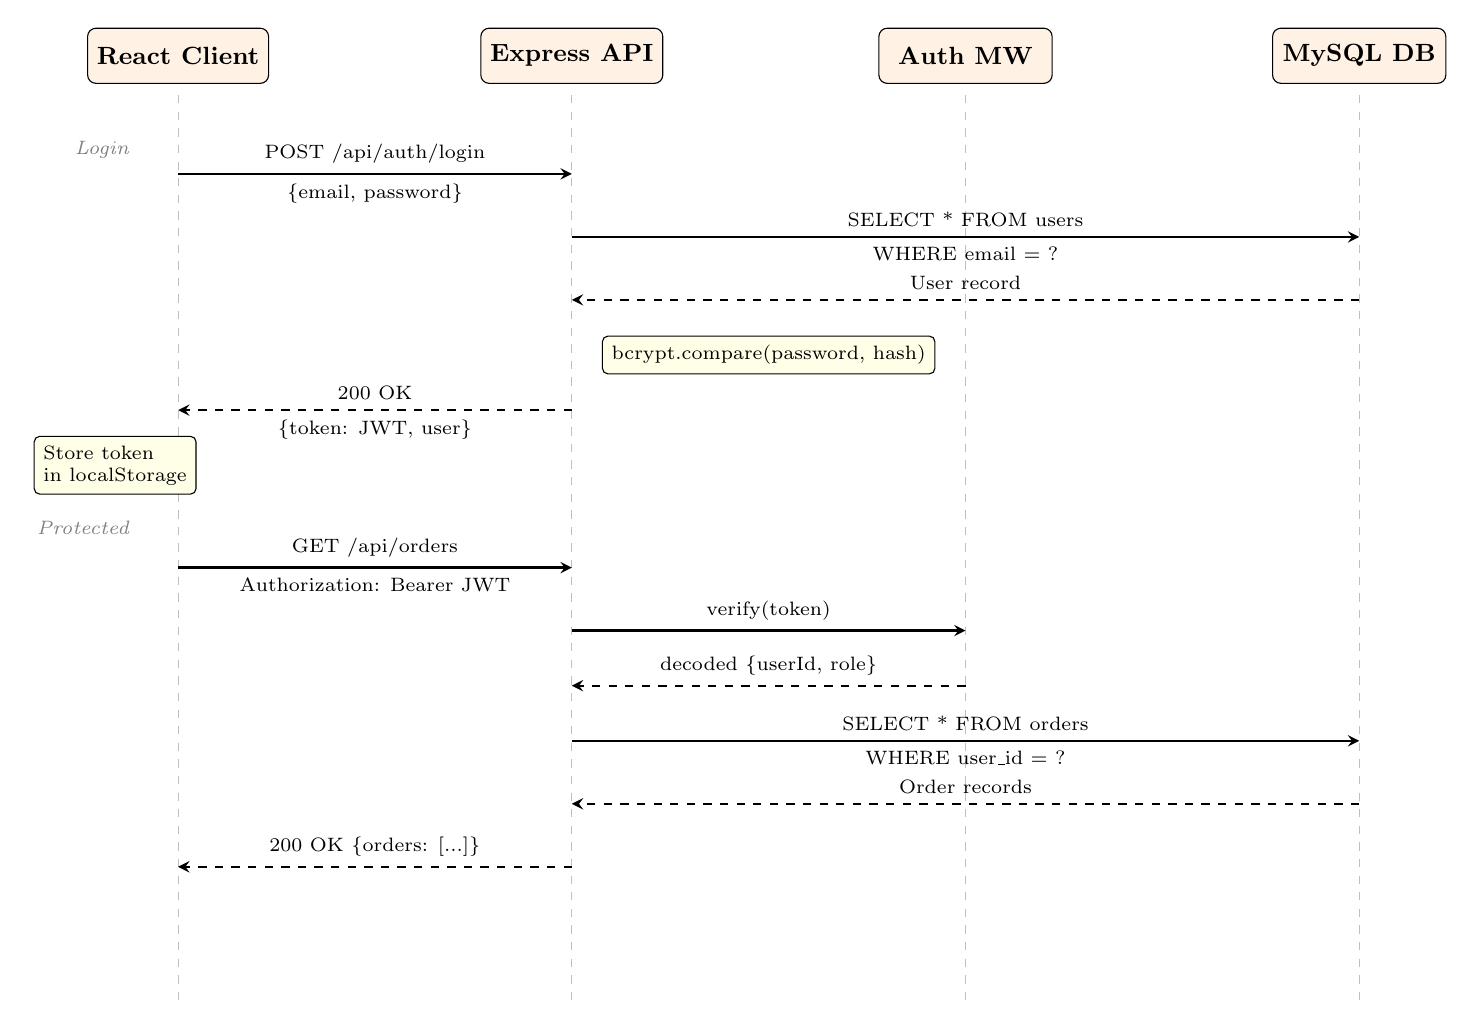
\begin{tikzpicture}[
  participant/.style={draw, rectangle, rounded corners=3pt, fill=orange!10, minimum width=2.2cm, minimum height=0.7cm, font=\small\bfseries},
  lifeline/.style={dashed, gray!50},
  msg/.style={->, thick, >=stealth},
  ret/.style={->, thick, >=stealth, dashed},
  note/.style={draw, fill=yellow!10, font=\scriptsize, rounded corners=2pt, align=left},
]
  % Participants
  \node[participant] (client) at (0,0) {React Client};
  \node[participant] (api) at (5,0) {Express API};
  \node[participant] (auth) at (10,0) {Auth MW};
  \node[participant] (db) at (15,0) {MySQL DB};

  % Lifelines
  \draw[lifeline] (0,-0.5) -- (0,-12);
  \draw[lifeline] (5,-0.5) -- (5,-12);
  \draw[lifeline] (10,-0.5) -- (10,-12);
  \draw[lifeline] (15,-0.5) -- (15,-12);

  % Login sequence
  \node[left, font=\scriptsize\itshape, gray] at (-0.5,-1.2) {Login};
  \draw[msg] (0,-1.5) -- node[above, font=\scriptsize] {POST /api/auth/login} node[below, font=\scriptsize] {\{email, password\}} (5,-1.5);
  \draw[msg] (5,-2.3) -- node[above, font=\scriptsize] {SELECT * FROM users} node[below, font=\scriptsize] {WHERE email = ?} (15,-2.3);
  \draw[ret] (15,-3.1) -- node[above, font=\scriptsize] {User record} (5,-3.1);

  \node[note] at (7.5,-3.8) {bcrypt.compare(password, hash)};

  \draw[ret] (5,-4.5) -- node[above, font=\scriptsize] {200 OK} node[below, font=\scriptsize] {\{token: JWT, user\}} (0,-4.5);

  \node[note] at (-0.8,-5.2) {Store token\\in localStorage};

  % Authenticated request
  \node[left, font=\scriptsize\itshape, gray] at (-0.5,-6.0) {Protected};
  \draw[msg] (0,-6.5) -- node[above, font=\scriptsize] {GET /api/orders} node[below, font=\scriptsize] {Authorization: Bearer JWT} (5,-6.5);
  \draw[msg] (5,-7.3) -- node[above, font=\scriptsize] {verify(token)} (10,-7.3);
  \draw[ret] (10,-8.0) -- node[above, font=\scriptsize] {decoded \{userId, role\}} (5,-8.0);
  \draw[msg] (5,-8.7) -- node[above, font=\scriptsize] {SELECT * FROM orders} node[below, font=\scriptsize] {WHERE user\_id = ?} (15,-8.7);
  \draw[ret] (15,-9.5) -- node[above, font=\scriptsize] {Order records} (5,-9.5);
  \draw[ret] (5,-10.3) -- node[above, font=\scriptsize] {200 OK \{orders: [...]\}} (0,-10.3);

\end{tikzpicture}
}
\caption{Sequence Diagram -- User Authentication Flow}
\label{fig:seq-auth}
\end{figure}

\subsection{Order Placement Flow}
Figure~\ref{fig:seq-order} shows the checkout and order creation sequence.

\begin{figure}[H]
\centering
\resizebox{\textwidth}{!}{
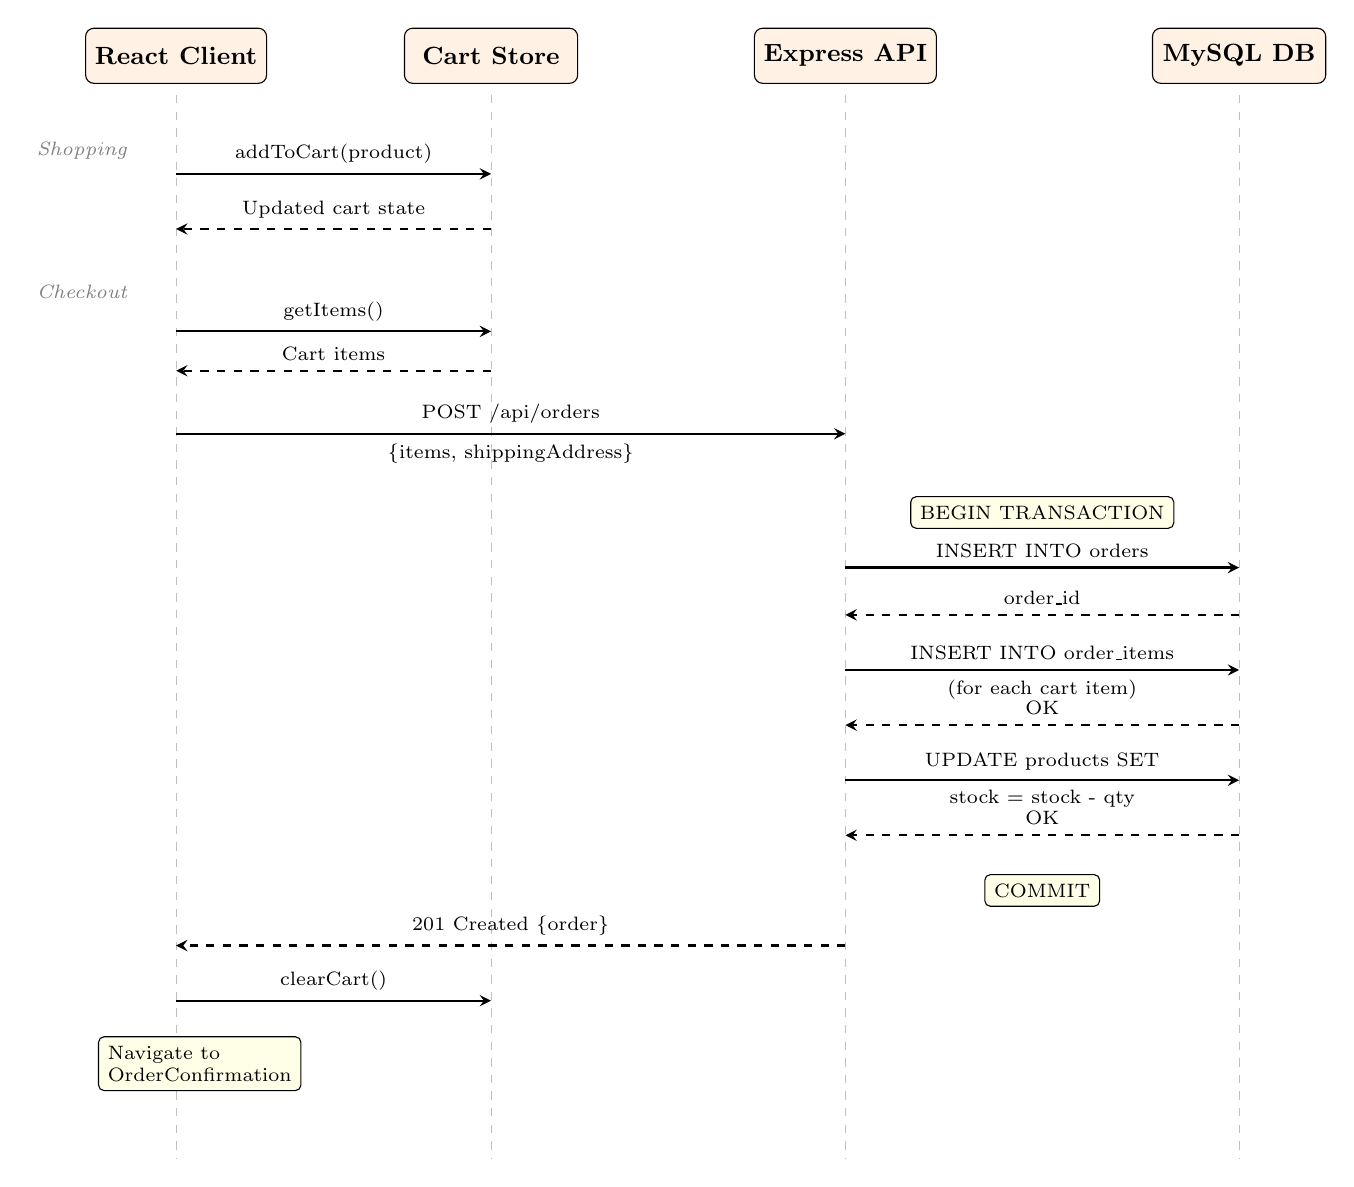
\begin{tikzpicture}[
  participant/.style={draw, rectangle, rounded corners=3pt, fill=orange!10, minimum width=2.2cm, minimum height=0.7cm, font=\small\bfseries},
  lifeline/.style={dashed, gray!50},
  msg/.style={->, thick, >=stealth},
  ret/.style={->, thick, >=stealth, dashed},
  note/.style={draw, fill=yellow!10, font=\scriptsize, rounded corners=2pt, align=left},
  activation/.style={draw, fill=orange!5, minimum width=0.4cm},
]
  % Participants
  \node[participant] (client) at (0,0) {React Client};
  \node[participant] (cart) at (4,0) {Cart Store};
  \node[participant] (api) at (8.5,0) {Express API};
  \node[participant] (db) at (13.5,0) {MySQL DB};

  % Lifelines
  \draw[lifeline] (0,-0.5) -- (0,-14);
  \draw[lifeline] (4,-0.5) -- (4,-14);
  \draw[lifeline] (8.5,-0.5) -- (8.5,-14);
  \draw[lifeline] (13.5,-0.5) -- (13.5,-14);

  % Add to cart (client-side)
  \node[left, font=\scriptsize\itshape, gray] at (-0.5,-1.2) {Shopping};
  \draw[msg] (0,-1.5) -- node[above, font=\scriptsize] {addToCart(product)} (4,-1.5);
  \draw[ret] (4,-2.2) -- node[above, font=\scriptsize] {Updated cart state} (0,-2.2);

  % Checkout
  \node[left, font=\scriptsize\itshape, gray] at (-0.5,-3.0) {Checkout};
  \draw[msg] (0,-3.5) -- node[above, font=\scriptsize] {getItems()} (4,-3.5);
  \draw[ret] (4,-4.0) -- node[above, font=\scriptsize] {Cart items} (0,-4.0);

  \draw[msg] (0,-4.8) -- node[above, font=\scriptsize] {POST /api/orders} node[below, font=\scriptsize] {\{items, shippingAddress\}} (8.5,-4.8);

  \node[note] at (11,-5.8) {BEGIN TRANSACTION};

  \draw[msg] (8.5,-6.5) -- node[above, font=\scriptsize] {INSERT INTO orders} (13.5,-6.5);
  \draw[ret] (13.5,-7.1) -- node[above, font=\scriptsize] {order\_id} (8.5,-7.1);

  \draw[msg] (8.5,-7.8) -- node[above, font=\scriptsize] {INSERT INTO order\_items} node[below, font=\scriptsize] {(for each cart item)} (13.5,-7.8);
  \draw[ret] (13.5,-8.5) -- node[above, font=\scriptsize] {OK} (8.5,-8.5);

  \draw[msg] (8.5,-9.2) -- node[above, font=\scriptsize] {UPDATE products SET} node[below, font=\scriptsize] {stock = stock - qty} (13.5,-9.2);
  \draw[ret] (13.5,-9.9) -- node[above, font=\scriptsize] {OK} (8.5,-9.9);

  \node[note] at (11,-10.6) {COMMIT};

  \draw[ret] (8.5,-11.3) -- node[above, font=\scriptsize] {201 Created \{order\}} (0,-11.3);

  \draw[msg] (0,-12.0) -- node[above, font=\scriptsize] {clearCart()} (4,-12.0);

  \node[note] at (0.3,-12.8) {Navigate to\\OrderConfirmation};

\end{tikzpicture}
}
\caption{Sequence Diagram -- Order Placement Flow}
\label{fig:seq-order}
\end{figure}

\section{API Endpoints}

\begin{longtable}{|l|l|l|p{4cm}|}
\caption{API Endpoint Reference} \label{tab:api} \\
\hline
\textbf{Method} & \textbf{Endpoint} & \textbf{Auth} & \textbf{Description} \\
\hline
\endfirsthead
\hline
\textbf{Method} & \textbf{Endpoint} & \textbf{Auth} & \textbf{Description} \\
\hline
\endhead
\hline
\endfoot

\multicolumn{4}{|c|}{\textbf{Authentication (/api/auth)}} \\
\hline
POST & /auth/register & -- & Register new user \\
POST & /auth/login & -- & Login, returns JWT \\
GET & /auth/profile & User & Get user profile \\
PUT & /auth/profile & User & Update profile \\
\hline

\multicolumn{4}{|c|}{\textbf{Products (/api/products)}} \\
\hline
GET & /products & -- & List products (paginated) \\
GET & /products/featured & -- & Get featured products \\
GET & /products/categories & -- & Get all categories \\
GET & /products/:id & -- & Get product by ID \\
POST & /products & Admin & Create product \\
PUT & /products/:id & Admin & Update product \\
DELETE & /products/:id & Admin & Delete product \\
GET & /products/:id/reviews & -- & Get product reviews \\
POST & /products/:id/reviews & User & Add review \\
\hline

\multicolumn{4}{|c|}{\textbf{Orders (/api/orders)}} \\
\hline
POST & /orders & User & Create order \\
GET & /orders & Admin & List all orders \\
GET & /orders/myorders & User & Get user's orders \\
GET & /orders/:id & User & Get order details \\
PUT & /orders/:id/status & Admin & Update order status \\
PUT & /orders/:id/confirm & Admin & Confirm order \\
PUT & /orders/:id/reject & Admin & Reject order \\
\hline

\multicolumn{4}{|c|}{\textbf{Users (/api/users)}} \\
\hline
GET & /users & Admin & List all users \\
GET & /users/:id & Admin & Get user by ID \\
PUT & /users/:id & Admin & Update user \\
DELETE & /users/:id & Admin & Delete user \\
\hline

\multicolumn{4}{|c|}{\textbf{Suppliers (/api/suppliers)}} \\
\hline
GET & /suppliers & -- & List active suppliers \\
GET & /suppliers/admin/all & Admin & List all suppliers \\
GET & /suppliers/:id & -- & Get supplier details \\
GET & /suppliers/:id/products & -- & Get supplier products \\
POST & /suppliers & Admin & Create supplier \\
PUT & /suppliers/:id & Admin & Update supplier \\
DELETE & /suppliers/:id & Admin & Delete supplier \\
\hline

\multicolumn{4}{|c|}{\textbf{Stats (/api/stats)}} \\
\hline
GET & /stats/dashboard & Admin & Dashboard statistics \\
\hline

\end{longtable}

\section{Request/Response Examples}

\begin{lstlisting}[language=JavaScript, caption={Login API -- Request and Response}]
// POST /api/auth/login
// Request Body:
{
  "email": "user@example.com",
  "password": "securePassword123"
}

// Response (200 OK):
{
  "token": "eyJhbGciOiJIUzI1NiIsInR5cCI6IkpXVCJ9...",
  "user": {
    "id": 1,
    "username": "john_doe",
    "email": "user@example.com",
    "role": "user"
  }
}
\end{lstlisting}

\begin{lstlisting}[language=JavaScript, caption={Products API -- List Response}]
// GET /api/products?limit=10&offset=0&sortBy=price&sortOrder=ASC
// Response (200 OK):
{
  "products": [
    {
      "id": 1,
      "name": "CyberStation Pro X1",
      "slug": "cyberstation-pro-x1",
      "price": 2999.99,
      "category_name": "Gaming Desktops",
      "supplier_name": "NVIDIA",
      "supplier_id": 1,
      "stock": 25,
      "rating": 4.80,
      "features": ["RTX 5090", "Intel i9-14900K"],
      "specifications": {"CPU": "Intel i9", "GPU": "RTX 5090"}
    }
  ]
}
\end{lstlisting}

\section{Error Handling}
All API errors follow a consistent format:
\begin{lstlisting}[language=JavaScript, caption={API Error Response Format}]
// 400 Bad Request
{ "message": "Product name is required" }

// 401 Unauthorized
{ "message": "Not authorized, token expired or invalid" }

// 403 Forbidden
{ "message": "Not authorized as admin" }

// 404 Not Found
{ "message": "Product not found" }

// 500 Internal Server Error
{ "message": "Server error", "error": "details..." }
\end{lstlisting}


% ======================= CHAPTER 8: USER INTERFACE =======================
\chapter{User Interface}

\section{Design Philosophy}
The application features a cyberpunk-themed dark UI design with the following characteristics:
\begin{itemize}[noitemsep]
  \item \textbf{Color Palette:} Dark backgrounds (\texttt{zinc-950}, \texttt{zinc-900}) with orange-400/500 accents and emerald status indicators.
  \item \textbf{Typography:} Bold, uppercase headers with tracking for a futuristic feel.
  \item \textbf{Animations:} Framer Motion for page transitions, hover effects, and loading states.
  \item \textbf{Components:} Rounded cards (\texttt{rounded-2xl/3xl}), glassmorphism effects, gradient overlays.
  \item \textbf{Responsiveness:} Mobile-first approach with Tailwind breakpoints (sm, md, lg, xl).
\end{itemize}

\section{Key Pages}

\subsection{Home Page}
Features a hero section with auto-sliding background images, featured products carousel, dynamic categories grid with subcategory hover dropdowns, statistics section, and newsletter subscription.

\subsection{Products Page}
Full product catalog with:
\begin{itemize}[noitemsep]
  \item Grid and list view toggle
  \item Category filtering sidebar
  \item Price range filtering
  \item Rating filtering
  \item Stock status filtering
  \item Sort by price, name, rating, newest
  \item Full-text search
  \item Pagination
\end{itemize}

\subsection{Product Detail Page}
Displays product image, name, price, rating with stars, supplier name (linked to supplier page), description, stock status, quantity selector, add to cart button, features list, specifications table, and a paginated reviews section with star rating submission.

\subsection{Shopping Cart}
Shows cart items with quantity adjustment, item removal, subtotal calculation, and checkout button. Cart state is persisted via Zustand's \texttt{persist} middleware.

\subsection{Admin Dashboard}
Tab-based administration panel with five sections:
\begin{enumerate}[noitemsep]
  \item \textbf{Overview:} Statistics cards (total sales, orders, users, products), recent orders list, low stock alerts, quick action buttons.
  \item \textbf{Products:} CRUD table with search, sort, pagination, edit/delete actions.
  \item \textbf{Orders:} Order list with status filters, status update, confirm/reject actions.
  \item \textbf{Users:} User management with role editing and account deletion.
  \item \textbf{Suppliers:} Supplier table with search, sort, toggle active/inactive, edit, delete with confirmation modal.
\end{enumerate}

\subsection{Supplier Pages}
\begin{itemize}[noitemsep]
  \item \textbf{Suppliers List:} Grid of supplier cards with search, sort, and country filtering.
  \item \textbf{Supplier Detail:} Full supplier info (contact, address, website), products grid with pagination.
  \item \textbf{Add/Edit Supplier:} Four-section form (Basic Info, Contact Person, Address, Financial \& Legal).
\end{itemize}

\section{Navigation}
The \texttt{CyberNavbar} component provides:
\begin{itemize}[noitemsep]
  \item Desktop mega-menu with product sub-categories
  \item Mobile hamburger menu with animated drawer
  \item Language toggle button (EN $\leftrightarrow$ AR)
  \item Cart icon with item count badge
  \item User dropdown (profile, orders, admin dashboard)
  \item Search bar
\end{itemize}

\section{Footer}
Global footer with:
\begin{itemize}[noitemsep]
  \item Newsletter subscription
  \item Quick links (Products, Categories, Suppliers)
  \item Support links
  \item Social media icons
  \item Copyright notice
\end{itemize}


% ======================= CHAPTER 9: TESTING =======================
\chapter{Testing and Evaluation}

\section{Testing Approach}
The project employs multiple testing strategies:

\subsection{API Testing}
Node.js scripts for end-to-end API testing:
\begin{itemize}[noitemsep]
  \item \texttt{api-test.js} -- General API endpoint testing
  \item \texttt{test-admin-login.js} -- Admin authentication testing
  \item \texttt{test-db.js} -- Database connectivity testing
  \item \texttt{scripts/e2e-review-http.js} -- End-to-end review creation via HTTP
  \item \texttt{scripts/test-review.js} -- Review system testing
\end{itemize}

\subsection{Database Testing}
\begin{itemize}[noitemsep]
  \item \texttt{scripts/list-products-direct.js} -- Direct database product queries
  \item \texttt{scripts/create-review-direct.js} -- Direct database review insertion
  \item \texttt{test-db.js} -- Connection pool and query testing
\end{itemize}

\subsection{Manual Testing}
Comprehensive manual testing was performed on:
\begin{itemize}[noitemsep]
  \item User registration and login flow
  \item Product browsing, filtering, and searching
  \item Shopping cart operations (add, remove, update quantity)
  \item Checkout and order placement
  \item Review submission and display
  \item Admin CRUD operations for all entities
  \item Supplier management (create, edit, toggle, delete)
  \item Language switching (EN $\leftrightarrow$ AR) and RTL layout
  \item Responsive design on mobile, tablet, and desktop viewports
\end{itemize}

\section{Test Results Summary}
\begin{table}[H]
\centering
\caption{Testing Results Summary}
\label{tab:testing}
\begin{tabularx}{\textwidth}{|l|X|l|}
\hline
\textbf{Module} & \textbf{Test Scope} & \textbf{Result} \\
\hline
Authentication & Register, login, JWT, admin access & Pass \\
Products & CRUD, search, filter, pagination & Pass \\
Orders & Create, list, status update & Pass \\
Users & Admin CRUD, role management & Pass \\
Suppliers & CRUD, toggle, product association & Pass \\
Reviews & Create, list, pagination & Pass \\
Cart & Add, remove, persist, checkout & Pass \\
i18n & EN/AR translations, RTL layout & Pass \\
Responsive & Mobile, tablet, desktop & Pass \\
API Security & Auth middleware, admin guard & Pass \\
Database & Connection pool, migrations & Pass \\
\hline
\end{tabularx}
\end{table}

\section{Performance Evaluation}
\begin{itemize}[noitemsep]
  \item \textbf{API Response Time:} Average $<$100ms for product listing queries.
  \item \textbf{Database Queries:} Optimized with indexes and connection pooling (10 concurrent connections).
  \item \textbf{Frontend Bundle:} Optimized with React production build and code splitting via React Router.
  \item \textbf{Image Handling:} Base64 upload with server-side file storage (max 10MB request body).
\end{itemize}


% ======================= CHAPTER 10: CONCLUSION =======================
\chapter{Conclusion and Future Work}

\section{Conclusion}
CyberStore successfully demonstrates the development of a comprehensive, full-stack e-commerce web application using modern technologies. The project achieves all stated objectives:

\begin{enumerate}[noitemsep]
  \item A fully functional e-commerce platform with 20+ pages and comprehensive admin tools.
  \item Secure authentication with JWT and role-based access control.
  \item A normalized MySQL database with 7 tables, foreign keys, indexes, and full-text search.
  \item Complete supplier management system integrated with the product catalog.
  \item Full bilingual support (English/Arabic) with 1,500+ translation keys and RTL layout.
  \item Product review and rating system.
  \item Responsive, animated UI with a cyberpunk design theme using Tailwind CSS and Framer Motion.
\end{enumerate}

The three-tier architecture (React frontend, Express backend, MySQL database) provides a clean separation of concerns, making the codebase maintainable and extensible. The auto-migration system ensures database schema consistency across deployments.

\section{Challenges Faced}
\begin{itemize}[noitemsep]
  \item \textbf{MySQL TEXT DEFAULT limitation:} MySQL does not allow DEFAULT values on TEXT columns, requiring schema adjustments (e.g., \texttt{address VARCHAR(500)} instead of \texttt{TEXT}).
  \item \textbf{Express route ordering:} Static routes like \texttt{/admin/all} must be registered before dynamic \texttt{/:id} routes to prevent parameter conflicts.
  \item \textbf{RTL layout:} Implementing full right-to-left support required careful handling of text alignment, margins, padding, and icon positioning across all components.
  \item \textbf{State synchronization:} Managing cart persistence and auth state across page reloads required careful Zustand middleware configuration.
\end{itemize}

\section{Future Work}
\begin{enumerate}[noitemsep]
  \item \textbf{Payment Gateway Integration:} Integrate Stripe or PayPal for real payment processing.
  \item \textbf{Email Notifications:} Order confirmation emails, password reset, and promotional newsletters.
  \item \textbf{Real-Time Features:} WebSocket integration for live order tracking and admin notifications.
  \item \textbf{Inventory Management:} Automated stock alerts and purchase order generation for suppliers.
  \item \textbf{Analytics Dashboard:} Sales charts, revenue trends, and customer behavior analytics.
  \item \textbf{Mobile Application:} React Native mobile app sharing the same API backend.
  \item \textbf{Image CDN:} Cloud-based image storage (AWS S3 / Cloudinary) for better performance.
  \item \textbf{Automated Testing:} Jest + React Testing Library for unit tests; Cypress for E2E tests.
  \item \textbf{Docker Deployment:} Containerized deployment with Docker Compose.
  \item \textbf{Search Engine:} Integrate Elasticsearch for advanced product search and suggestions.
\end{enumerate}


% ======================= REFERENCES =======================
\chapter*{References}
\addcontentsline{toc}{chapter}{References}

\begin{enumerate}[label={[\arabic*]}, noitemsep]
  \item Facebook/Meta, ``React -- A JavaScript Library for Building User Interfaces,'' \url{https://react.dev/}, 2024.
  \item Express.js, ``Express -- Node.js Web Application Framework,'' \url{https://expressjs.com/}, 2024.
  \item MySQL, ``MySQL 8.0 Reference Manual,'' \url{https://dev.mysql.com/doc/refman/8.0/en/}, 2024.
  \item React Router, ``React Router v6 Documentation,'' \url{https://reactrouter.com/}, 2024.
  \item Tailwind Labs, ``Tailwind CSS Documentation,'' \url{https://tailwindcss.com/docs}, 2024.
  \item Zustand, ``Zustand -- Bear Necessities for State Management,'' \url{https://zustand-demo.pmnd.rs/}, 2024.
  \item JSON Web Tokens, ``Introduction to JSON Web Tokens,'' \url{https://jwt.io/introduction}, 2024.
  \item Framer, ``Framer Motion -- Production-Ready Animations for React,'' \url{https://www.framer.com/motion/}, 2024.
  \item Axios, ``Axios -- Promise Based HTTP Client,'' \url{https://axios-http.com/}, 2024.
  \item Lucide, ``Lucide Icons -- Beautiful Consistent Icons,'' \url{https://lucide.dev/}, 2024.
  \item Node.js Foundation, ``Node.js Documentation,'' \url{https://nodejs.org/en/docs/}, 2024.
  \item bcryptjs, ``bcrypt.js -- Optimized bcrypt in JavaScript,'' \url{https://www.npmjs.com/package/bcryptjs}, 2024.
\end{enumerate}

\end{document}
